\newpage
\section{\seamlessmodel}
\label{sec:unified}
In this section, we introduce \seamlessmodel,
which combines two derivatives of \mfourttwo, namely 
\seamlessexpressive—an offline translation model with comprehensive prosody preservation—and
\seamlessstreaming—a multilingual streaming speech-to-speech translation model—to engender a unified system that provides real time and expressive S2ST.
To the best of our knowledge, \seamlessmodel marks the first, publicly available system of its kind, paving the way for a myriad of downstream possibilities that can help those experiencing language barriers better communicate in the wild.

Notably, \seamlessmodel maintains the same semantic accuracy and latency shown in \seamlessstreaming.
In addition, \seamless captures a key expressivity transfer features from \seamlessexpressive. More specifically, it focuses to preserve sentence-level expressivity, e.g., tone, emotional expression and the style of one's voice rather than phrase-level one, e.g., speech rate and pauses.
Based on preliminary user testing, it does not appear that not offering the full suite of expressive preservation impacted the overall experience of our test subjects.






\begin{figure}[!ht]
    \centering
    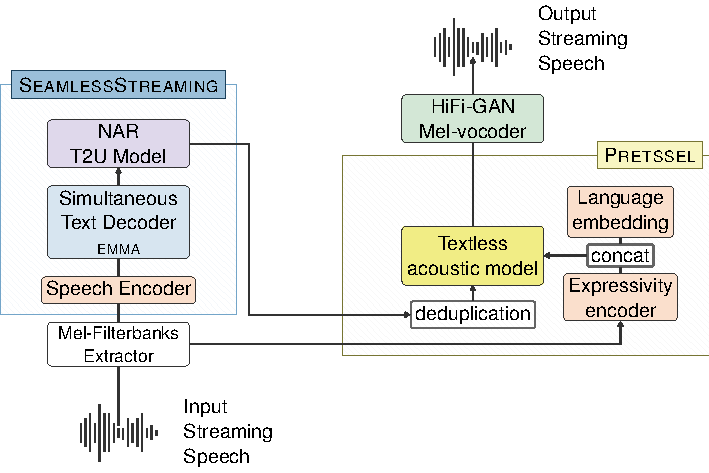
\includegraphics[width=0.6\linewidth]{figures/seamless.pdf}
    \caption{The architecture of \seamlessmodel.}
    \label{fig:seamless_arch_overview}
\end{figure}
\subsection{Architecture}
\Cref{fig:seamless_arch_overview} provides an overview of the architecture for the \seamlessmodel model.
First, \seamlessstreaming generates streaming text and discrete units from source speech.
\seamlessstreaming, empowered by EMMA and NAR T2U model, can be quickly adapted from the large-scale trained foundational \mfourttwo, as described in \Cref{sec:streaming}.
Then, the generated units are fed into the expressive speech generator, \ptv to preserve the sentence-level prosody and the style of one's voice from the partial source speech.
Finally, the synthesized Mel-filterbank features from the textless acoustic model will be fed to the HiFi-GAN vocoder to produce expressive translated speech in real-time.

The base version of \ptv in \seamlessexpressive supports six high-resource languages. In order to study the behavior of this unified architecture when language support is further scaled, we also trained a version of \ptv with an extended set of 36 languages and tested it with \seamlessmodel. Details on language coverage and training data statistics can be found in \Cref{app:ptvextdata}.

We present two versions of \seamlessmodel—\seamless-6 and \seamlessmodel-36.
While \seamless-6 shares \seamlessexpressive's coverage for high-resource languages, %
\seamlessmodel-36 extends its language coverage to that of \seamlessstreaming by leveraging the language-extended \ptv model. %

\subsection{Results and Discussion}
We only conducted automatic evaluations on the \seamlessmodel.
\subsubsection{\ptv extension}
We report the automatic measurement of \ptv trained with different data.
We document the offline performance of two different \ptv models, 
namely \ptv-6\footnote{Note that this model is same \ptv model used for \seamlessexpressive.} and \ptv-36, in \Cref{tbl:seamless.offline.p2v}. 
As evidenced by the results, English output remains of similar quality overall. The significantly expanded set of languages does, however, come at the cost of lowering performance for non-English target languages, as measured by ASR-BLEU and vocal style similarity. Overall, results demonstrate the feasibility of broad language support for \ptv, although a larger model might be required for increased capacity.

\begin{table}[!tbh]
    \centering
    \begin{tabular}{@{}lcccccc@{}}
        \toprule
         \makecell[c]{\textbf{Metrics}}  
         & \multicolumn{2}{c}{\makecell[c]{\xeng \\{\it (n=101)}}} 
         & \multicolumn{2}{c}{\makecell[c]{\engx \\{\it (n=5)}}} 
         & \multicolumn{2}{c}{\makecell[c]{\engx \\{\it (n=35)}}} \\
         \midrule
         \makecell[c]{\ptv \\ Language Coverage} & 6 & 36 & 6 & 36 & 6 & 36 \\
          \midrule
         \makecell[c]{ASR-BLEU}&  25.8 &  25.5&  29.3 &  28.3&  --&  22.78\\
         \makecell[c]{Vocal Style Similarity} &  0.30 &  0.30&  0.24 &  0.19 &  --&  0.18\\
         \makecell[c]{\comparator} &  2.35 &  2.46&  2.80&  2.88&  --&  2.86\\
        \bottomrule
    \end{tabular}
    \caption{The automatic measurement on \fleurs of the \ptv models trained on six and 36 languages. The middle column compares results for the \engx direction limited to the five non-English languages supported by \seamlessexpressive.}
    \label{tbl:seamless.offline.p2v}
\end{table}

\subsubsection{Quality-latency} 
Similar to \seamlessstreaming,
we report translation quality and latency under different decision thresholds $t_{\emma}$ \footnote{For details, see \Cref{sec:streaming.results.quality}} 
in \Cref{tbl:seamless_s2s.latency-quality.xeng} and \Cref{tbl:seamless_s2s.latency-quality.engx}. 
We can see that the model has a small degradation from \seamlessstreaming on ASR-BLEU in both \xeng and \engx directions.
\seamless has a lower ending offset, which means the \ptv model can generate speech with a shorter duration.
\seamless-6 has better performance for \seamlessexpressive's six target language directions than \seamless-36, while \seamless-36 has the same coverage as \seamlessstreaming.
The full results and metrics per evaluation direction can be found here: \url{https://github.com/facebookresearch/seamless_communication}.
\begin{table}[H]
    \centering
    \small
    \begin{tabular}{@{}lccc@{}}
        \toprule
         \multirow{4}{*}{\bf Model}  &   \multirow{4}{*}{\makecell[c]{{\bf  Decision} \\  \bf{Threshold}}}  & \multicolumn{2}{c}{\makecell[c]{\xeng \\{\it (n=101)}}} \\
         \cmidrule{3-4}
         & & ASR-BLEU & \makecell[c]{Ending \\ Offset}  \\
         \midrule
\multirow{4}{*}{\seamlessstreaming}  
 & 0.4 & 21.8 & 2.66 \\
 & 0.5 & 22.1 & 2.79 \\
 & 0.6 & 22.0 & 2.81 \\
 & 0.7 & 22.0 & 2.91 \\
        \midrule
     \multirow{4}{*}{\seamless-6}  
 & 0.4 & 20.3 & 1.95 \\
 & 0.5 & 20.4 & 2.02 \\
 & 0.6 & 20.5 & 2.09 \\
 & 0.7 & 20.7 & 2.15 \\
    \midrule
    \multirow{4}{*}{\seamless-36}  
 & 0.4 & 17.8 & 2.00 \\
 & 0.5 & 18.1 & 2.09 \\
 & 0.6 & 18.3 & 2.17 \\
 & 0.7 & 18.6 & 2.26 \\
        \bottomrule
    \end{tabular}
    \caption{Average translation quality and latency of \seamless under different latency decision threshold $t_{\emma}$ on \fleurs, to English directions. }
    \label{tbl:seamless_s2s.latency-quality.xeng}
\end{table}

\begin{table}[!tbh]
    \centering
    \small
    \begin{tabular}{@{}lccccc@{}}
        \toprule
         \multirow{4}{*}{\bf Model}  &   \multirow{4}{*}{\makecell[c]{{\bf  Decision} \\  \bf{Threshold}}}  & \multicolumn{2}{c}{\makecell[c]{\engx \\{\it (n=5)}}} & \multicolumn{2}{c}{\makecell[c]{\engx\\{\it (n=35)}}} \\
         \cmidrule(r){3-4}\cmidrule(l){5-6}
         & & ASR-BLEU & \makecell[c]{Ending \\ Offset} & ASR-BLEU & \makecell[c]{Ending \\ Offset} \\
         \midrule
\multirow{4}{*}{\seamlessstreaming}  
& 0.4 & 27.7 & 4.11 & 20.8 & 4.59 \\
& 0.5 & 27.8 & 4.15 & 21.4 & 4.64 \\
& 0.6 & 27.9 & 4.20 & 21.5 & 4.69 \\
& 0.7 & 28.0 & 4.25 & 21.6 & 4.73 \\
        \midrule
 \multirow{4}{*}{\seamless-6}  
 & 0.4 & 25.6 & 2.77 & --- & ---\\
& 0.5 & 25.6 & 2.83  & --- & ---\\
  & 0.6 & 25.7 & 2.88 & --- & ---\\
& 0.7 & 25.8 & 2.95 & --- & ---\\
        \midrule
        \multirow{4}{*}{\seamless-36}  
        & 0.4 & 23.4 & 2.81  & 16.1 & 3.38 \\
        & 0.5 & 23.4 & 2.87 & 16.2 & 3.43 \\
        & 0.6 & 23.6 & 2.93 & 16.1 & 3.49 \\
        & 0.7 & 23.7 & 2.99 & 16.3 & 3.55 \\    
        \bottomrule
    \end{tabular}
    \caption{Average translation quality and latency of \seamless under different latency decision threshold $t_{\emma}$ on \fleurs. The column with $(n=5)$ compares the results for the eng–X direction limited to
the 5 non-English languages supported by \seamlessexpressive.}
    \label{tbl:seamless_s2s.latency-quality.engx}
\end{table}

\subsubsection{Expressivity preservation}
We present the expressivity preservation at different latency in \Cref{tbl:seamless.s2s.exp.xeng} and \Cref{tbl:seamless.s2s.exp.engx}.
Comparing with \Cref{tbl:seamless.offline.p2v},
there is a degration in both vocal style similarity and \comparator due to the partial context used in \ptv.
\begin{table}[H]
    \centering
    \small
    \begin{tabular}{@{}lcccc@{}}
        \toprule
         \multirow{4}{*}{\bf Model}  &   \multirow{4}{*}{\makecell[c]{{\bf  Decision} \\  \bf{Threshold}}}  & \multicolumn{2}{c}{\makecell[c]{\xeng \\{\it (n=101)}}} \\
         \cmidrule{3-5}
         & & \makecell[c]{Vocal Style \\ Similarity} 
          & \makecell[c]{\comparator}
          & \makecell[c]{Ending \\ Offset}   \\
         \midrule
     \multirow{4}{*}{\seamless-6}  
 & 0.4 & 0.21 & 1.89 & 1.95 \\
 & 0.5 & 0.21 & 1.89 & 2.02 \\
 & 0.6 & 0.21 & 1.89 & 2.09 \\
 & 0.7 & 0.21 & 1.90 & 2.15 \\

    \midrule
    \multirow{4}{*}{\seamless-36}  
 & 0.4 & 0.22 & 1.76 & 2.01 \\
 & 0.5 & 0.23 & 1.76 & 2.10 \\
 & 0.6 & 0.23 & 1.77 & 2.17 \\
 & 0.7 & 0.23 & 1.78 & 2.26 \\
        \bottomrule
    \end{tabular}
    \caption{Average expressivity preservation and latency measurements of \seamless under different latency decision threshold $t_{\emma}$ on \fleurs, to English Directions.
    }
    \label{tbl:seamless.s2s.exp.xeng}
\end{table}

\begin{table}[!tbh]
    \centering
    \small
    \begin{tabular}{@{}lccccccc@{}}
        \toprule
             \multirow{4}{*}{\bf Model}
             & \multirow{4}{*}{\makecell[l]{{\bf  Decision} \\  \bf{Threshold}} } & \multicolumn{3}{c}{\makecell[c]{\engx \\{\it (n=5)}}} & \multicolumn{3}{c}{\makecell[c]{\engx\\{\it (n=35)}}} \\
         \cmidrule(r){3-5}\cmidrule(l){6-8}
          & & \makecell[c]{Vocal Style \\ Similarity} 
          & \makecell[c]{\comparator}
          & \makecell[c]{Ending \\ Offset} 
          & \makecell[c]{Vocal Style \\ Similarity} 
          & \makecell[c]{\comparator }
          & \makecell[c]{Ending \\ Offset} \\
         \midrule 
\multirow{4}{*}{\seamless-6} 
& 0.4 & 0.18 & 2.48 & 2.77 & --- & --- & --- \\
& 0.5 & 0.18 & 2.49 & 2.83 & --- & --- & --- \\
& 0.6 & 0.18 & 2.49 & 2.88 & --- & --- & --- \\
& 0.7 & 0.18 & 2.49 & 2.95 & --- & --- & --- \\
 \midrule
 \multirow{4}{*}{\seamless-36} 
 & 0.4 & 0.19 & 2.38 & 2.81 &0.19 & 2.36 & 3.38\\
 & 0.5 & 0.19 & 2.39 & 2.87  &  0.19 & 2.36 & 3.43 \\
& 0.6 & 0.19 & 2.39 & 2.93 & 0.19 & 2.37 & 3.49 \\
& 0.7 & 0.19 & 2.39 & 2.99 & 0.19 & 2.37 & 3.55 \\
        \bottomrule
    \end{tabular}
    \caption{Average expressivity preservation and latency measurements of \seamless under different latency decision threshold $t_{\emma}$ on \fleurs.
    The column with $(n=5)$ compares the results for the eng–X direction limited to
the 5 non-English languages supported by \seamlessexpressive.}
    \label{tbl:seamless.s2s.exp.engx}
\end{table}
\FloatBarrier
\newpage